%%
%% ****** ljmsamp.tex 13.06.2018 ******
%%
\documentclass[
11pt,%
tightenlines,%
twoside,%
onecolumn,%
nofloats,%
nobibnotes,%
nofootinbib,%
superscriptaddress,%
noshowpacs,%
centertags]%
{revtex4-2}
\usepackage{ljm}
\begin{document}

\titlerunning{Sufficient Sample Size Estimation: Likelihood Bootstrapping} % for running heads
\authorrunning{Nikita Kiselev, Andrey Grabovoy} % for running heads
%\authorrunning{First-Author, Second-Author} % for running heads

\title{Sufficient Sample Size Estimation:\\ Likelihood Bootstrapping}
% Splitting into lines is performed by the command \\
% The title is written in accordance with the rules of capitalization.

\author{\firstname{N.~S.}~\surname{Kiselev}}
\email[E-mail: ]{kiselev.ns@phystech.edu}
\affiliation{Moscow Institute of Physics and Technology, 9 Institutskiy per., Dolgoprudny, Moscow Region, 141701, Russian Federation}

\author{\firstname{A.\,V.}~\surname{Grabovoy}}
\email[E-mail: ]{grabovoy.av@phystech.edu}
\affiliation{Moscow Institute of Physics and Technology, 9 Institutskiy per., Dolgoprudny, Moscow Region, 141701, Russian Federation}
%\noaffiliation % If the author does not specify a place of work.

%\firstcollaboration{(Submitted by A.~A.~Editor-name)} % Add if you know submitter.
%\lastcollaboration{ }

%\received{June 13, 2018} % The date of receipt to the editor, i.e. December 06, 2017


\begin{abstract} % You shouldn't use formulas and citations in the abstract.
    The paper investigates the problem of estimating a sufficient sample size. The issue of determining a sufficient sample size without specifying a statistical hypothesis about the distribution of model parameters is considered. Two approaches to determining a sufficient sample size based on likelihood function values on resampled subsets are proposed. These approaches are based on heuristics about the behavior of the likelihood function with a large number of objects in the sample. A method for forecasting the likelihood function in case of an insufficient sample size is proposed. A computational experiment is conducted to analyze the properties of the proposed methods.
\end{abstract}

%\subclass{12345, 54321} % Enter 2010 Mathematics Subject Classification.

\keywords{Sufficient sample size, Likelihood bootstrapping, Genetic algorithm, Linear regression} % Include keywords separeted by comma.

\maketitle

% Text of article starts here.

% ====================
\section{Introduction}
% ====================

The process of supervised machine learning entails the selection of a predictive model from a family of parametric models, a decision often based on specific statistical assumptions, such as optimizing a particular quality function. A model that aligns with these statistical assumptions is termed as a \textit{adequate} model \cite{bies2006genetic, cawley2010over, raschka2018model}.

In the planning phase of a computational experiment, it is crucial to estimate the minimum required sample size, which refers to the number of objects necessary to construct a suitable model. The sample size needed to develop an adequate predictive model is called \textit{sufficient} \cite{byrd2012sample, figueroa2012predicting, balki2019sample}. 

This study focuses on the determination of a sufficient sample size, a topic that has been extensively researched with methods categorized into statistical, Bayesian, and heuristic approaches.

Early investigations on this subject, such as \cite{Adcock1988, Joseph1995}, establish a specific statistical criterion, where the sample size estimation method associated with this criterion guarantees achieving a fixed statistical power with a Type I error not exceeding a specified value. Statistical methods include the Lagrange multipliers test \cite{self1988power}, the Likelihood ratio test \cite{shieh2000power}, the Wald statistic \cite{shieh2005power}. Statistical methods have certain limitations associated with their practical application. They enable the estimation of the sample size based on assumptions about data distribution and information regarding the consistency of observed values with the assumptions of the null hypothesis.

The Bayesian method is another approach to this problem. In the study \cite{Lindley1997}, the sufficient sample size is ascertained by maximizing the expected utility function, which may explicitly incorporate parameter distribution functions and penalties for increasing the sample size. This study also explores alternative methods based on restricting a certain quality criterion for model parameter estimation. Notable among these criteria are the Average Posterior Variance Criterion (APVC), Average Coverage Criterion (ACC), Average Length Criterion (ALC), and Effective Sample Size Criterion (ESC). These criteria have been further refined in subsequent research, such as \cite{PhamGia1997} and \cite{Gelfand2002}. Eventually, the authors of \cite{Cao2009} conducted a theoretical and practical comparison of methods from \cite{Adcock1988, Joseph1995, Lindley1997}.

Researchers like \cite{Brutti2014} and \cite{Pezeshk2008} delve into the distinctions between Bayesian and frequentist approaches in determining sample size, proposing robust methods for the Bayesian approach and providing illustrative examples for certain probabilistic models.

The paper \cite{Grabovoy2022} examines various methods for sample size estimation in generalized linear models, encompassing statistical, heuristic, and Bayesian methods. Techniques such as Lagrange Multiplier Test, Likelihood Ratio Test, Wald Test, Cross-Validation, Bootstrap, Kullback-Leibler Criterion, Average Posterior Variance Criterion, Average Coverage Criterion, Average Length Criterion, and Utility Maximization are analyzed. The authors highlight the potential of combining Bayesian and statistical approaches to estimate sample size when available sample sizes are insufficient.

In \cite{MOTRENKO2014743}, a method for determining sample size in logistic regression is presented, utilizing cross-validation and Kullback-Leibler divergence between posterior distributions of model parameters on similar subsamples. Similar subsamples refer to those that can be derived from each other by adding, removing, or replacing one object.

The genetic algorithm, as described in \citep{Goldberg1988}, can be employed to approximate a given set of functions. This algorithm represents an optimization process where a population of candidates (known as individuals) evolves towards superior solutions \citep{Mirjalili2019}. Each individual possesses a set of characteristics (genes or phenotypes) that can evolve over time. Evolution occurs through crossover or mutation operations. The evolution commences with a random population, with each generation serving as the foundation for the next one. The fitness of individuals is assessed in each generation, and individuals with superior fitness are chosen to create a new generation \citep{Kramer2017}. The algorithm concludes after reaching the maximum number of generations or achieving satisfactory results, resulting in each new generation becoming more adapted to the environment.

This paper discusses several approaches to determining a sufficient sample size. It is proposed to estimate the mathematical expectation and variance of the likelihood function on bootstrapped subsamples. A small change in these values when adding another object indicates that a sufficient number of objects in the sample has been reached. The correctness of the definition in the linear regression model is proved. The presented method is easy to use in practice. To do this, it is proposed to calculate the value of the loss function instead of the likelihood. The paper also proposes a method that allows you to estimate a sufficient sample size if there are not enough objects. A genetic algorithm is used to approximate a large number of dependencies of the error function on the sample size on open datasets with regression and classification tasks.

% =========================
\section{Problem statement}
% =========================

An object is defined as a pair $(\mathbf{x}, y)$, where $\mathbf{x} \in \mathbb{X} \subseteq \mathbb{R}^n$ is the feature vector, and $y \in \mathbb{Y}$ is the target variable. In regression problems $\mathbb{Y} = \mathbb{R}$, and in $K$-class classification problems $\mathbb{Y} = \{1, \ldots, K\}$.

The feature-object matrix for a sample $\mathfrak{D}_m = \left\{ (\mathbf{x}_i, y_i) \right\}, i \in \mathcal{I} = \{ 1, \ldots, m \}$ of size $m$ is called the matrix $\mathbf{X}_m = \left[ \mathbf{x}_1, \ldots, \mathbf{x}_m \right]^{\top} \in \mathbb{R}^{m \times n}$.

The target variable vector for a sample $\mathfrak{D}_m = \left\{ (\mathbf{x}_i, y_i) \right\}, i \in \mathcal{I} = \{ 1, \ldots, m \}$ of size $m$ is denoted by $\mathbf{y}_m = \left[ y_1, \ldots, y_m \right]^{\top} \in \mathbb{Y}^m$.

A model is a parametric family of functions $f$, mapping the Cartesian product of the set of feature vector values $\mathbb{X}$ and the set of parameter values $\mathbb{W}$ to the set of target variable values $\mathbb{Y}$: 
\[ f: \mathbb{X} \times \mathbb{W} \to \mathbb{Y}. \]

A probabilistic model is a joint distribution
\[ p(y, \mathbf{w} | \mathbf{x}) = p(y | \mathbf{x}, \mathbf{w}) p(\mathbf{w}): \mathbb{Y} \times \mathbb{W} \times \mathbb{X} \to \mathbb{R}^+, \]
where $\mathbf{w} \in \mathbb{W}$ is the set of model parameters, $p(y | \mathbf{x}, \mathbf{w})$ specifies the likelihood of an object, and $p(\mathbf{w})$ represents the prior distribution of parameters.

The likelihood function of a sample $\mathfrak{D}_m = \left\{ (\mathbf{x}_i, y_i) \right\}, i \in \mathcal{I} = \{ 1, \ldots, m \}$ of size $m$, where $\mathbf{x}_1, \ldots, \mathbf{x}_m$ are i.i.d. together, is defined as 
\[ L(\mathfrak{D}_m, \mathbf{w}) = p(\mathbf{y}_m | \mathbf{X}_m, \mathbf{w}) = \prod_{i=1}^{m} p(y_i | \mathbf{x}_i, \mathbf{w}). \]
Its logarithm
\[ l(\mathfrak{D}_m, \mathbf{w}) = \sum\limits_{i=1}^{m} \log p(y_i | \mathbf{x}_i, \mathbf{w}) \]
is called the logarithmic likelihood function. Unless stated otherwise, we consider samples to be i.i.d.

The maximum likelihood estimate of a set of parameters $\mathbf{w} \in \mathbb{W}$ based on the subsample $\mathfrak{D}_k$ of size $k$ is given by 
\[ \hat{\mathbf{w}}_{k} = \arg\max_{\mathbf{w} \in \mathbb{W}} L(\mathfrak{D}_k, \mathbf{w}). \]

The task is to determine the sufficient sample size $m^*$. Let a criterion $T$ be given. E.g. it can be constructed based on heuristics regarding the behaviour of model parameters.
\begin{definition}
    The sample size $m^*$ is called \textbf{sufficient} according to the criterion $T$, if $T$ holds for all $k \geqslant m^*$.
\end{definition}
It should be noted that it is possible for $m^* \leqslant m$ or $m^* > m$. These two cases will be considered separately later on.

% ============================================================================
\section{Sufficient sample size does not exceed the available one}\label{sec2}
% ============================================================================

In this section, we will assume that $m^*\leqslant m$ is valid. This means that we just need to formalize which sample size can be considered sufficient. To determine sufficiency, we will use the likelihood function. When there are enough objects available, it is quite natural to expect that the resulting parameter estimate will not change much from one sample realization to another \cite{Joseph1997, Joseph1995}. The same can be said about the likelihood function. Thus, we formulate which sample size can be considered sufficient.

\begin{definition}
    \label{sufficient-variance}
    Let's fix some positive number $\varepsilon > 0$. The sample size $m^*$ is called \textbf{D-sufficient} if for all $k\geqslant m^*$
    \[ D(k) = \mathbb{D}_{\hat{\mathbf{w}}_{k}} L(\mathfrak{D}_m, \hat{\mathbf{w}}_{k}) \leqslant \varepsilon. \]
\end{definition}

On the other hand, when there are enough objects available, it is also quite natural that when adding another object to consideration, the resulting parameter estimate will not change much. Let's formulate another definition.

\begin{definition}
    \label{sufficient-difference}
    Let's fix some positive number $\varepsilon > 0$. The sample size $m^*$ is called \textbf{M-sufficient} if for all $k\geqslant m^*$ 
    \[ M(k) = \left| \mathbb{E}_{\hat{\mathbf{w}}_{k+1}} L(\mathfrak{D}_m, \hat{\mathbf{w}}_{k+1}) - \mathbb{E}_{\hat{\mathbf{w}}_{k}} L(\mathfrak{D}_m, \hat{\mathbf{w}}_{k}) \right| \leqslant \varepsilon. \]
\end{definition}
In the definitions above instead of the likelihood function $L(\mathfrak{D}_m, \hat{\mathbf{w}}_{k})$ we can consider its logarithm $l(\mathfrak{D}_m, \hat{\mathbf{w}}_{k})$.

Suppose that $\mathbb{W} = \mathbb{R}^n$. Recall that the Fisher information is called the matrix
\[ \left[\mathcal{I}(\mathbf{w})\right]_{ij} = - \mathbb{E}\left[ \dfrac{\partial^2 \log p(\mathbf{y} | \mathbf{x}, \mathbf{w})}{\partial w_i \partial w_j} \right]. \]
A known result is the asymptotic normality of the maximum likelihood estimate, that is, $\sqrt{k}\left(\hat{\mathbf{w}}_k -\mathbf{w}\right)\xrightarrow{d}\mathcal{N}\left(0, \mathcal{I}^{-1}(\mathbf{w})\right)$. Convergence in the distribution generally does not imply convergence of the moments of a random vector. Nevertheless, if we assume the latter, then in some models it is possible to prove the correctness of our proposed definition of M-sufficient sample size.

For convenience, we denote the distribution parameters $\hat{\mathbf{w}}_k$ as follows: mathematical expectation $\mathbb{E}\hat{\mathbf{w}}_k=\mathbf{m}_k$ and the covariance matrix $\mathbb{D} \hat{\mathbf{w}}_k = \mathbf{\Sigma}_k$. Then the following theorem holds, the proof of which is given in the section \ref{append}.

\begin{theorem}\label{theorem1}
    Let $\|\mathbf{m}_{k+1} - \mathbf{m}_k\|_2 \to 0$ and $\|\mathbf{\Sigma}_{k+1} - \mathbf{\Sigma}_k\|_{F}\to 0$ as $k\to \infty$. Then, in the linear regression model, the definition of M-sufficient sample size is correct. Namely, for any $\varepsilon > 0$, there is such a $m^*$ that for all $k\geqslant m^*$ $M(k)\leqslant\varepsilon$ is satisfied.
\end{theorem}

\begin{corollary}
    Let $\|\mathbf{m}_k - \mathbf{w}\|_2\to 0$ and $\|\mathbf{\Sigma}_k - \left[k\mathcal{I}(\mathbf{w})\right]^{-1}\|_{F}\to 0$ for $k \to \infty$. Then, in the linear regression model, the definition of an M-sufficient sample size is correct. 
\end{corollary}

By condition, one sample is given. Therefore, in the experiment it is not possible to calculate the mathematical expectation and variance specified in the definitions. To evaluate them, we will use the bootstrap technique. Namely, we will generate from the given $\mathfrak{D}_m$ a number of $B$ subsamples of size $k$ with a return. For each of them, we get an estimate of the parameters $\hat{\mathbf{w}}_{k}$ and calculate the value of $L(\mathfrak{D}_m, \hat{\mathbf{w}}_{k})$. For the estimation, we will use a sample mean and an unbiased sample variance (for bootstrap samples).

The definitions proposed above can also be applied in those problems where an arbitrary loss function is minimized rather than the likelihood function is maximized. We do not provide any theoretical justification for this, but in practice such a heuristic turns out to be quite successful.

% ===================================================================
\section{Sufficient sample size is larger than available}\label{sec3}
% ===================================================================

In this section, we will assume that $m^*> m$ is valid.

The problem arises of predicting the mathematical expectation of the likelihood function / loss function at $k > m$. In general, this is quite a difficult task. In this paper, it is proposed to analyze a large number of open datasets from \citep{UCI} in order to find a parametric family of functions that should approximate the dependence of the loss function on the sample size used. It is proposed to study datasets with regression and classification tasks separately.

One of the simplest search algorithms in terms of implementation and logic is the genetic algorithm. Using it, we will build a method for finding the desired family of functions. 

Suppose that for $N$ different datasets, a graph is plotted of the dependence of the average value of the loss function (or likelihood function with a minus sign) on the sample size used. Let's bring these $N$ dependencies to the same scale on both axes. To do this, subtract the minimum value, and then divide by the maximum value. In this case, the graph of each dependence is squared $[0; 1]^2$, It starts at the point $(0; 1)$ and ends at the point $(1; 0)$.

A population in a genetic algorithm is a set of parametric families of functions.
For example, one individual can be a family of $w_0 + w_1\cdot\log(w_2\cdot x) + w_3\cdot x^2$, where $x$ is a variable, and $\mathbf{w}$ is a vector of parameters. The initial population is initialized randomly. The simplest unary functions are used: $1, x, \sin{x}, \cos{x}, \exp{x}, \log{x}, \ctg{x}$ and $\cth{x}$, as well as the simplest binary functions: $+, -, *$ and $/$. Each individual is represented using a binary tree, the nodes of which contain the above-mentioned functions, and the leaves are necessarily $1$ or $x$. At the same time, each node is assigned its own component of the parameter vector.

The fitness of an individual is measured as follows. For each of the $N$ approximated dependencies, the problem of selecting a vector of parameters is solved. The mean squared error is minimized. The resulting MSE value is averaged over all $N$ dependencies. The final value determines the fitness of the individual.

The crossover is implemented in such a way that a random subtree of one of the parent individuals is replaced by a random subtree of the other. A mutation replaces a function in a random node of the tree with another random function. 

The algorithm terminates after a given number of generations. An individual from the last generation with the best fitness is selected. The solution is an appropriate parametric family of functions.

% ============================================
\section{Computational experiment}\label{sec4}
% ============================================

An experiment has been conducted to analyze the properties of the proposed methods for estimating a sufficient sample size. The experiment consists of several parts. In the first part, estimates of a sufficient sample size are considered in the case when a sufficient sample size does not exceed the available one. The second part examines the results obtained under the conditions that a sufficient sample size is larger than the available one.

% -------------------------------------------------------------------
\subsection{Sufficient sample size does not exceed the available one}
% -------------------------------------------------------------------

% ...................................................
\subsubsection{Convergence of the proposed functions}
% ...................................................

Synthetic data is generated from a linear regression model. The number of objects is 1000, the number of features is 20. $B=100$ bootstrap samples were used. As a result, for each sample size $k$, the values of the functions $D(k)$ and $M(k)$ defined in Chapter~\ref{sec2} are obtained (the logarithm of the likelihood function is used here). The following is a Fig.~\ref{synthetic-regression-functions}, which shows the resulting dependencies.

\begin{figure}[h!]
    \centering
    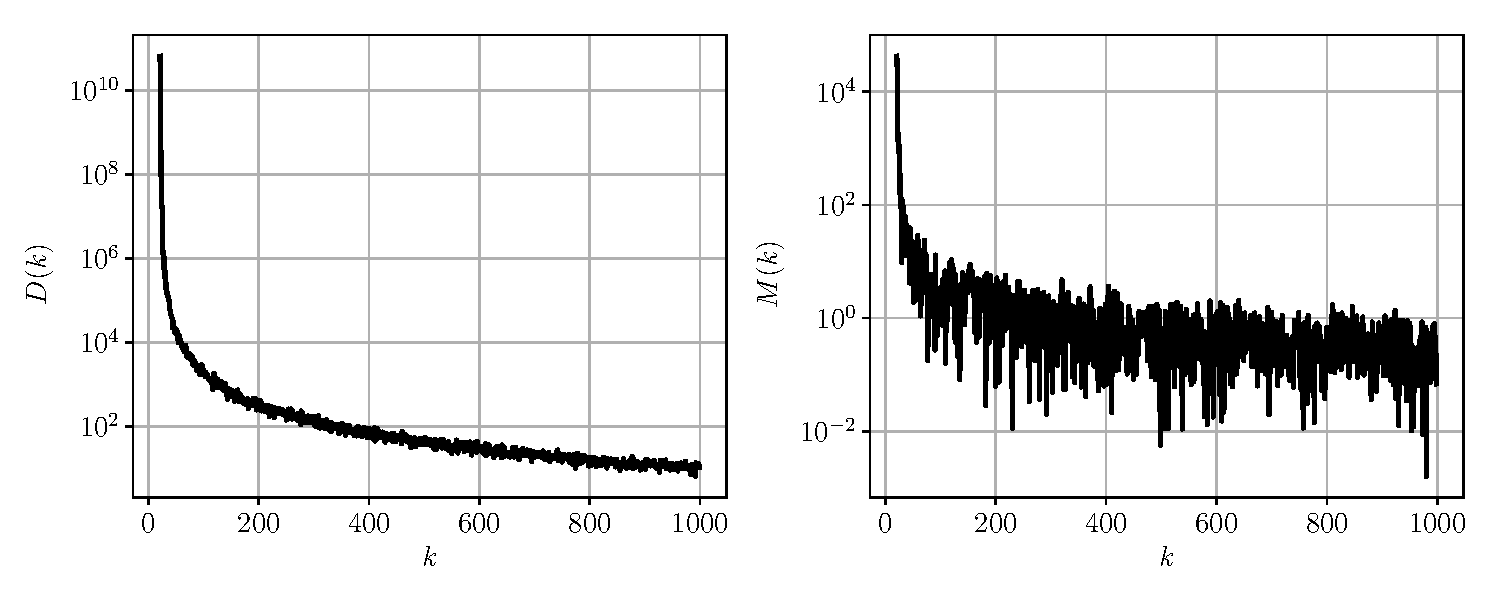
\includegraphics[width=0.9\textwidth]{../paper/figures/gray/eps/synthetic-regression-functions-D-M}
    \caption{Convergence of functions for synthetic sample (linear regression)}
    \label{synthetic-regression-functions}
\end{figure}

The graphs obtained confirm the results obtained in the Theorem~\ref{theorem1}. The values of the functions $D(k)$ and $M(k)$ tend to zero as the size of the subsample increases. 

% ..................................................
\subsubsection{Determining a sufficient sample size}
% ..................................................

Synthetic data is generated from a linear regression model. The number of objects is 1000, the number of features is 20. The following are graphs of the logarithm of the likelihood function of the sample, as well as the functions $D(k)$ and $M(k)$ for the logarithm of the likelihood function. $B=1000$ bootstrap samples were used. The definition of D-sufficient and M-sufficient sample sizes has been performed. For D-sufficiency, $\varepsilon = 3 \cdot 10^{1}$ is selected, for M-sufficiency $\varepsilon = 4 \cdot 10^{-1}$. The results are shown in Fig.~\ref{synthetic-regression-sufficient}. 

\begin{figure}[h!]
    \centering
    \includegraphics[width=\textwidth]{../paper/figures/gray/eps/synthetic-regression-sufficient}
    \caption{Synthetic sample (linear regression) at $m^*\leqslant m$}
    \label{synthetic-regression-sufficient}
\end{figure}

The second synthetic sample is generated from a logistic regression model. The number of objects is 1000, the number of features is 20. Similar graphs are shown in Fig.~\ref{synthetic-classification-sufficient}. For D-sufficiency, $\varepsilon = 3 \cdot 10^1$ was used, for M-sufficiency $\varepsilon = 6 \cdot 10^{-1}$.

\begin{figure}[h!]
    \centering
    \includegraphics[width=\textwidth]{../paper/figures/gray/eps/synthetic-classification-sufficient}
    \caption{Synthetic sample (logistic regression) at $m^* \leqslant m$}
    \label{synthetic-classification-sufficient}
\end{figure}

The following is an example of determining a sufficient sample size based on real data. The Abalone dataset from \citep{UCI} is used with the regression task. The number of objects is 4177, the number of features is 8. The results are shown in Fig.~\ref{abalone-sufficient}. The definition of D-sufficiency uses $\varepsilon=2.5 \cdot 10^{-3}$, for M-sufficiency, $\varepsilon=8 \cdot 10^{-3}$ is taken.

\begin{figure}[h!]
    \centering
    \includegraphics[width=\textwidth]{../paper/figures/gray/eps/abalone-sufficient}
    \caption{Abalone sample (regression) at $m^*\leqslant m$}
    \label{abalone-sufficient}
\end{figure}

% ------------------------------------------------------------------
\subsection{Sufficient sample size is larger than the available one}
% ------------------------------------------------------------------

% .........................................................................................
\subsubsection{Determination of a parametric family of functions using a genetic algorithm}
% .........................................................................................

The implementation of the genetic algorithm given in the section \ref{sec3} can be found in the repository \texttt{https://github.com/kisnikser/Bayesian-Sample-Size-Estimation}. To analyze the dependence of the loss function on the sample size used in the regression task, the following datasets from \citep{UCI} were used: Abalone, Auto MPG, Liver Disorders, Wine Quality, Parkinsons Telemonitoring, Bike Sharing Dataset, Real estate valuation and Heart failure clinical records. The quadratic loss function MSE was chosen. The regression problem for each of them was solved using linear regression from \citep{scikit-learn}. Averaging was performed on $B = 100$ bootstrap samples. As mentioned earlier, all dependencies are reduced to the same scale on both axes. The resulting graphs are shown in Fig.~\ref{datasets-regression}. On the left is a graph for the sample average. On the right is a graph for the sample standard deviation.

\begin{figure}[h!]
    \centering
    \includegraphics[width=\textwidth]{../paper/figures/gray/eps/datasets-regression}
    \caption{Behavior of the loss function in the regression problem}
    \label{datasets-regression}
\end{figure}

The application of the genetic algorithm leads to the same family of functions for approximating the mean and standard deviation in the regression problem:
\[ w_0 + w_1 \cdot \exp(w_2 \cdot x). \]

The classification task used 12 datasets from \citep{UCI}: Automobile, Breast Cancer Wisconsin (Diagnostic), Car Evaluation, Credit Approval, Glass Identification, Ionosphere, Iris, Tic-Tac-Toe Endgame, Congressional Voting Records, Wine, Zoo and Heart failure clinical records. The classification problem for each of them was solved using logistic regression from \citep{scikit-learn}. Averaging was performed on $B = 100$ bootstrap samples. All the curves are also reduced to the same scale on both axes. The resulting graphs are shown in Fig.~\ref{datasets-classification}. As before, there is a graph for the sample mean on the left, and a graph for the sample standard deviation on the right.

\begin{figure}[h!]
    \centering
    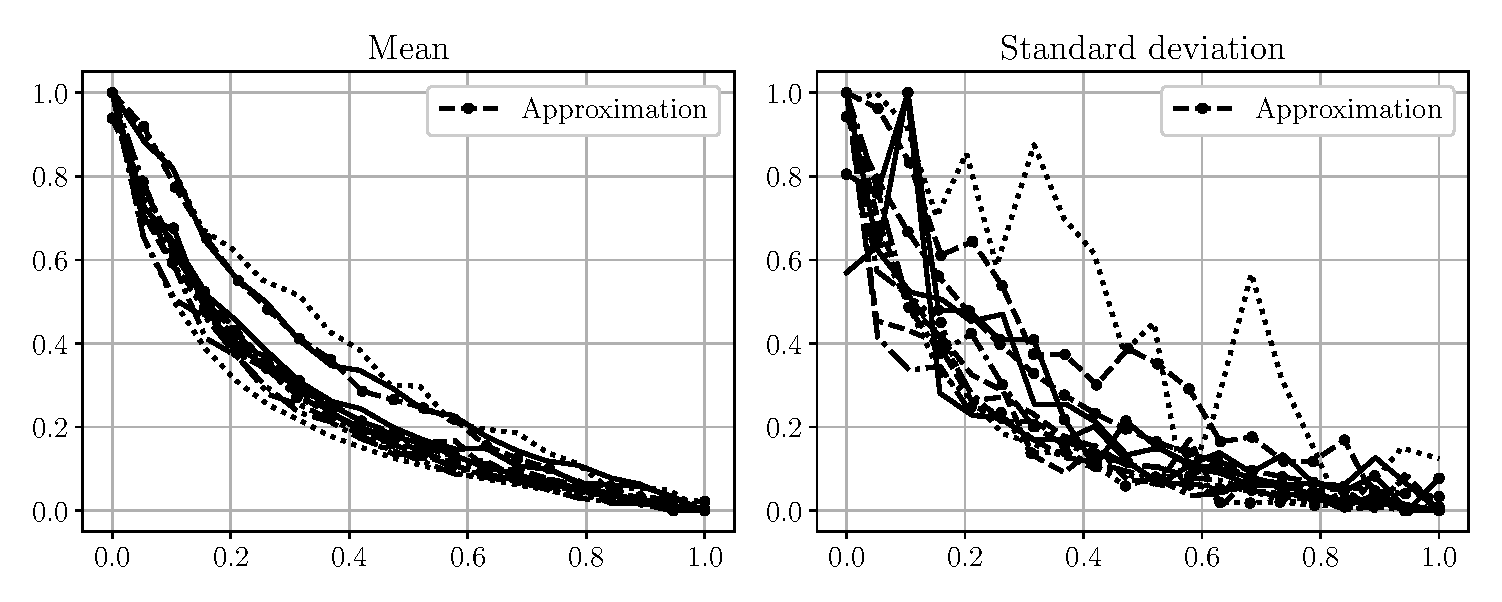
\includegraphics[width=\textwidth]{../paper/figures/gray/eps/datasets-classification}
    \caption{Behavior of the loss function in the classification problem}
    \label{datasets-classification}
\end{figure}

The application of a genetic algorithm for the mean value leads to the same family of functions as in the regression problem:
\[ w_0 + w_1 \cdot \exp(w_2 \cdot x). \]

The standard deviation in the case of a classification problem for each sample has its own dependence on the sample size. Thus, predicting variance for classification turns out to be quite a difficult task.

% ...................................................
\subsubsection{Prediction of the likelihood function}
% ...................................................

For synthetic samples, the approximation of likelihood functions is carried out. The mean and variance are approximated by the parametric family of functions given in the previous paragraph.

The division into training and test samples was carried out in the ratio of 70:30. The approximation was performed only on the training part. A sufficient sample size was in the test part. In Fig.~\ref{synthetic-regression-approximation} and Fig.~\ref{synthetic-classification-approximation} the true and approximated dependencies for synthetic data are presented. It also indicates the sample sizes determined by the true dependence D-sufficient and M-sufficient. 

\begin{figure}[h!]
    \centering
    \includegraphics[width=\textwidth]{../paper/figures/gray/eps/synthetic-regression-approximation}
    \caption{Synthetic sample (linear regression) at $m^*> m$}
    \label{synthetic-regression-approximation}
\end{figure}

\begin{figure}[h!]
    \centering
    \includegraphics[width=\textwidth]{../paper/figures/gray/eps/synthetic-classification-approximation}
    \caption{Synthetic sample (logistic regression) at $m^*> m$}
    \label{synthetic-classification-approximation}
\end{figure}

Next, similar results were obtained for the Abalone sample from \citep{UCI}. They are shown in Fig.~\ref{abalone-approximation}.

\begin{figure}[h!]
    \centering
    \includegraphics[width=\textwidth]{../paper/figures/gray/eps/abalone-approximation}
    \caption{Abalone sample (regression) at $m^* > m$}
    \label{abalone-approximation}
\end{figure}

% ==================
\section{Conclusion}
% ==================

Approaches to determining a sufficient sample size based on the proximity of posterior distributions of model parameters on similar subsamples are proposed. The correctness of the proposed approaches is proved under certain restrictions on the model used. The theorem on the moments of the limit posterior distribution of parameters in a linear regression model is proved. The conducted computational experiment makes it possible to analyze the properties of the proposed methods and their effectiveness.

\appendix

% ========================================
\section{Proofs of theorems}\label{append}
% ========================================

\begin{proof}[Proof (Theorem \ref{theorem1})]
Consider the definition of an M-sufficient sample size in terms of the logarithm of the likelihood function. In a linear regression model
    \[ L\left( \mathfrak{D}_m, \hat{\mathbf{w}}_k \right) = p(\mathbf{y} | \mathbf{X}, \hat{\mathbf{w}}_k) = \prod_{i=1}^{m} p(y_i | \mathbf{x}_i, \hat{\mathbf{w}}_k) = \prod_{i=1}^{m} \mathcal{N}\left( y_i | \hat{\mathbf{w}}_k^{\top} \mathbf{x}_i, \sigma^2 \right) = \]
    \[= \left(2\pi\sigma^2 \right)^{-m/2} \exp\left(-\dfrac{1}{2\sigma^2}\|\mathbf{y} -\mathbf{X} \hat{\mathbf{w}}_k\|_2^2 \right). \]
Take a logarithm:
    \[ l\left( \mathfrak{D}_m, \hat{\mathbf{w}}_k \right) = \log p(\mathbf{y} | \mathbf{X}, \hat{\mathbf{w}}_k) = -\dfrac{m}{2}\log\left( 2\pi\sigma^2 \right) - \dfrac{1}{2\sigma^2} \| \mathbf{y} - \mathbf{X} \hat{\mathbf{w}}_k \|_2^2. \]
Let's take the mathematical expectation of $\mathfrak{D}_k$, given that $\mathbb{E}_{\mathfrak{D}_k}\hat{\mathbf{w}}_k=\mathbf{m}_k$ and $\text{cov}(\hat{\mathbf{w}}_k) = \mathbf{\Sigma}_k$:
    \[ \mathbb{E}_{\mathfrak{D}_k} l\left( \mathfrak{D}_m, \hat{\mathbf{w}}_k \right) = -\dfrac{m}{2}\log\left( 2\pi\sigma^2 \right) - \dfrac{1}{2\sigma^2} \Big( \| \mathbf{y} - \mathbf{X} \mathbf{m}_k \|_2^2 + \text{tr}\left( \mathbf{X}^{\top}\mathbf{X} \mathbf{\Sigma}_k \right) \Big). \]
    Let's write down an expression for the difference in mathematical expectations:
    \[ \mathbb{E}_{\mathfrak{D}_{k+1}} l(\mathfrak{D}_m, \hat{\mathbf{w}}_{k+1}) - \mathbb{E}_{\mathfrak{D}_k} l(\mathfrak{D}_m, \hat{\mathbf{w}}_{k}) = \]
    \[ = \dfrac{1}{2\sigma^2} \Big( \| \mathbf{y} - \mathbf{X} \mathbf{m}_k \|_2^2 - \| \mathbf{y} - \mathbf{X} \mathbf{m}_{k+1} \|_2^2 \Big) + \dfrac{1}{2\sigma^2} \text{tr} \Big( \mathbf{X}^{\top}\mathbf{X} \left( \mathbf{\Sigma}_k - \mathbf{\Sigma}_{k+1} \Big) \right) = \]
    \[ = \dfrac{1}{2\sigma^2} \Big( 2 \mathbf{y}^{\top} \mathbf{X} (\mathbf{m}_{k+1} - \mathbf{m}_k) + (\mathbf{m}_k - \mathbf{m}_{k+1})^{\top} \mathbf{X}^{\top}\mathbf{X} (\mathbf{m}_k + \mathbf{m}_{k+1}) \Big) + \]
    \[ + \dfrac{1}{2\sigma^2} \text{tr} \Big( \mathbf{X}^{\top}\mathbf{X} \left( \mathbf{\Sigma}_k - \mathbf{\Sigma}_{k+1} \right) \Big). \]
The value of the function $M(k)$ is a module from the above expression. Let's apply the triangle inequality for the module, and then evaluate each term.\\
We estimate the first term using the Cauchy-Schwarz inequality:
\[\big| \mathbf{y}^{\top}\mathbf{X}(\mathbf{m}_{k+1}-\mathbf{m}_k)\big| \leqslant \| \mathbf{X}^{\top}\mathbf{y} \|_2 \|\mathbf{m}_{k+1} - \mathbf{m}_k\|_2. \]
    The second term is estimated using the Cauchy-Schwarz inequality, the consistency property of the spectral matrix norm, as well as the limitation of the sequence of vectors $\mathbf{m}_k$, which follows from the presented convergence condition:
\[\big| (\mathbf{m}_k - \mathbf{m}_{k+1})^{\top} \mathbf{X}^{\top}\mathbf{X} (\mathbf{m}_k + \mathbf{m}_{k+1}) \big| \leqslant \| \mathbf{X} (\mathbf{m}_k - \mathbf{m}_{k+1}) \|_2 \| \mathbf{X} (\mathbf{m}_k + \mathbf{m}_{k+1}) \|_2 \leqslant \]
    \[ \leqslant \| \mathbf{X} \|_2^2 \| \mathbf{m}_k - \mathbf{m}_{k+1} \|_2 \| \mathbf{m}_k + \mathbf{m}_{k+1} \|_2 \leqslant C \| \mathbf{X} \|_2^2 \| \mathbf{m}_k - \mathbf{m}_{k+1} \|_2. \]
    We estimate the last term using the Holder's inequality for the Frobenius norm:
    \[ \Big| \text{tr} \Big( \mathbf{X}^{\top}\mathbf{X} \left( \mathbf{\Sigma}_k - \mathbf{\Sigma}_{k+1} \right) \Big) \Big| \leqslant \| \mathbf{X}^{\top}\mathbf{X} \|_F \| \mathbf{\Sigma}_k - \mathbf{\Sigma}_{k+1} \|_F. \]
Finally, since $\|\mathbf{m}_k - \mathbf{m}_{k+1} \|_2\to 0$ and $\|\mathbf{\Sigma}_k - \mathbf{\Sigma}_{k+1}\|_{F}\to 0$ as $k\to\infty$, then $M(k)\to 0$ as $k\to \infty$, which proves the theorem.
\end{proof}

\begin{proof}[Proof (Corollary)]
    From the convergence conditions given, it follows that $\|\mathbf{m}_k - \mathbf{m}_{k+1} \|_2\to 0$ and $\|\mathbf{\Sigma}_k -\mathbf{\Sigma}_{k+1}\|_{F}\to 0$ for $k\to \infty$. The application of the \ref{theorem1} theorem completes the proof.
\end{proof}

%
% The Bibliography
%

\begin{thebibliography}{99}

\bibitem{bies2006genetic}
R.~R.~Bies, M.~F.~Muldoon, B.~G.~Pollock, S.~Manuck, G.~Smith, and M.~E.~Sale. \textquotedblleft A genetic algorithm-based, hybrid machine learning approach to model selection, \textquotedblright Journal of pharmacokinetics and pharmacodynamics, \textbf{33} (2), 195 (2006).

\bibitem{cawley2010over}
G.~C.~Cawley and N.~L.~Talbot. \textquotedblleft On over-fitting in model selection and subsequent selection bias in performance evaluation, \textquotedblright The Journal of Machine Learning Research, \textbf{11}, 2079--2107 (2010).

\bibitem{raschka2018model}
S.~Raschka. \textquotedblleft Model evaluation, model selection, and algorithm selection in machine learning, \textquotedblright arXiv preprint arXiv:1811.12808 (2018).

\bibitem{byrd2012sample}
R.~H.~Byrd, G.~M.~Chin, J.~Nocedal, and Y.~Wu. \textquotedblleft Sample size selection in optimization methods for machine learning, \textquotedblright Mathematical programming, \textbf{134} (1), 127--155 (2012).

\bibitem{figueroa2012predicting}
R.~L.~Figueroa, Q.~Zeng-Treitler, S.~Kandula, and L.~H.~Ngo. \textquotedblleft Predicting sample size required for classification performance, \textquotedblright BMC medical informatics and decision making, \textbf{12}, 1--10 (2012).

\bibitem{balki2019sample}
I.~Balki et al. \textquotedblleft Sample-size determination methodologies for machine learning in medical imaging research: a systematic review, \textquotedblright Canadian Association of Radiologists Journal, \textbf{70}(4), 344--353 (2019).

\bibitem{Adcock1988}
C.~J.~Adcock. \textquotedblleft A Bayesian approach to calculating sample sizes,\textquotedblright Journal of the Royal Statistical Society: Series D (The Statistician) \textbf{37} (4-5), 433--439 (1988).

\bibitem{Joseph1995}
L.~Joseph, D.~B.~Wolfson, and R.~D.~Berger. \textquotedblleft Sample size calculations for binomial proportions via highest posterior density intervals,\textquotedblright Journal of the Royal Statistical Society. Series D (The Statistician), \textbf{44}(2), 143--154 (1995).

\bibitem{self1988power}
S.~G.~Self and R.~H.~Mauritsen. \textquotedblleft Power/sample size calculations for generalized linear models, \textquotedblright Biometrics, 79--86 (1988).

\bibitem{shieh2000power}
G.~Shieh. \textquotedblleft On power and sample size calculations for likelihood ratio tests in generalized linear models, \textquotedblright Biometrics, \textbf{56}(4), 1192--1196 (2000).

\bibitem{shieh2005power}
G.~Shieh. \textquotedblleft On power and sample size calculations for wald tests in generalized linear models, \textquotedblright Journal of Statistical Planning and Inference, \textbf{128}(1), 43--59 (2005).

\bibitem{Lindley1997}
D.~V.~Lindley. \textquotedblleft The choice of sample size,\textquotedblright Journal of the Royal Statistical Society: Series D (The Statistician), \textbf{46}(2), 129--138 (1997).

\bibitem{PhamGia1997}
T.~Pham-Gia. \textquotedblleft On bayesian analysis, bayesian decision theory and the sample size problem,\textquotedblright Journal of the Royal Statistical Society: Series D (The Statistician), \textbf{46}(2), 139--144 (1997).

\bibitem{Gelfand2002}
A.~E.~Gelfand and F.~Wang. \textquotedblleft A simulation-based approach to bayesian sample size determination for performance under a given model and for separating models,\textquotedblright Statistical Science, \textbf{17} (2), (2002).

\bibitem{Cao2009}
J.~Cao, J.~J.~Lee, and S.~Alber. \textquotedblleft Comparison of bayesian sample size criteria: Acc, alc, and woc,\textquotedblright Journal of Statistical Planning and Inference, \textbf{139}(12), 4111--4122 (2009).

\bibitem{Brutti2014}
P.~Brutti, F.~De Santis, and S.~Gubbiotti. \textquotedblleft Bayesian-frequentist sample size determination: a game of two priors,\textquotedblright METRON, \textbf{72}(2), 133--151 (2014).

\bibitem{Pezeshk2008}
H.~Pezeshk, N.~Nematollahi, V.~Maroufy, and J.~Gittins. \textquotedblleft The choice of sample size: a mixed bayesian / frequentist approach,\textquotedblright Statistical Methods in Medical Research, \textbf{18}(2), 183--194 (2008).

\bibitem{Grabovoy2022}
A.~V.~Grabovoy, T.~T.~Gadaev, A.~P.~Motrenko, and V.~V.~Strijov. \textquotedblleft Numerical methods of sufficient sample size estimation for generalised linear models,\textquotedblright Lobachevskii Journal of Mathematics, \textbf{43}(9), 2453--2462 (2022).

\bibitem{MOTRENKO2014743}
A.~Motrenko, V.~Strijov, and G.-W.~Weber. \textquotedblleft Sample size determination for logistic regression,\textquotedblright Journal of Computational and Applied Mathematics, \textbf{255}, 743--752 (2014).

\bibitem{Goldberg1988}
D.~E. Goldberg and J.~H.~Holland. \textquotedblleft Genetic algorithms and machine learning,\textquotedblright Machine Learning, \textbf{3}(2), 95--99 (1988).

\bibitem{Mirjalili2019}
S.~Mirjalili. \textquotedblleft Genetic algorithm,\textquotedblright Evolutionary Algorithms and Neural Networks: Theory and Applications, 43--55 (2019).

\bibitem{Kramer2017}
O.~Kramer. \textquotedblleft Genetic Algorithms,\textquotedblright Springer International Publishing, 11--19 (2017).

\bibitem{Aduenko2017}
A.~A.~Aduenko. \textquotedblleft Selection of multimodels in classification tasks,\textquotedblright Ph.d. diss., Moscow (2017).

\bibitem{UCI}
K.~Markelle, L.~Rachel, and N.~Kolby. \textquotedblleft The UCI machine learning repository. \textquotedblright

\bibitem{scikit-learn}
F.~Pedregosa et. al. \textquotedblleft Scikit-learn: Machine learning in Python,\textquotedblright Journal of Machine Learning Research, \textbf{12}, 2825--2830 (2011).

\end{thebibliography}

\end{document}
